\chapter{原子轨道：形状、能量与大小}\label{ch:b2:atomic-orbitals}

氢原子没有边界：电子可能出现在离原子核任意远处，
其概率迅速下降，但永远不会降为零。
然而原子有大小，钠原子的宽度约为
氯原子的两倍，尽管它所含的电子更少。本科一年级分册用
三个量子数描述电子的状态；这里每个量子数都化为
位置的函数，具有形状、节面、符号与大小，并由一组简单的
规则把它们转化为任意原子的轨道能量。这些形状与符号
正是后面四章组合成分子轨道的内容。

\begin{recall}
本科一年级分册：量子数 $n$、$l$、$m_l$、$m_s$；将原子轨道视为
状态 $(n, l, m_l)$；电子层与电子亚层；屏蔽与有效核
电荷（定性）；电子排布；氢原子的能级，
$-E_R/n^2$，其中 $E_R = \qty{13.6}{eV}$。物理学中的波函数，
其模的平方即概率密度。
\end{recall}

\section{氢原子的波函数}

\begin{definition}[波函数]\label{def:b2:atomic-orbitals:wavefunction}
电子的状态由\emph{波函数}\index{波函数}
$\psi(x, y, z)$ 描述；$|\psi|^2$ 为其\emph{概率密度}\index{概率密度}：
电子出现在某点附近小体积 $dV$ 内的概率
为 $|\psi|^2\,dV$，且 $\int|\psi|^2\,dV = 1$（在全空间上积分），
即该函数已归一化。原子轨道是原子中单个电子的
波函数。
\end{definition}

\begin{definition}[径向部分与角向部分]\label{def:b2:atomic-orbitals:radial-angular}
在以原子核为中心的球坐标 $(r, \theta, \varphi)$ 下，类氢原子的轨道
可分解为 $\psi_{nlm}(r, \theta, \varphi) = R_{nl}(r)\,
Y_{lm}(\theta, \varphi)$：\emph{径向部分}\index{径向部分} $R_{nl}$ 仅依赖于 $n$ 与 $l$，
\emph{角向部分}\index{角向部分} $Y_{lm}$ 仅依赖于 $l$ 与
$m_l$。
\end{definition}

\begin{theorem}[类氢轨道]\label{thm:b2:atomic-orbitals:hydrogen}
对于核电荷为 $Ze$ 的单电子原子，取 $\rho = Zr/a_0$，$a_0 =
\qty{52.9}{pm}$ 为玻尔半径，$n \leq 3$ 时的径向部分如下，
以 $(Z/a_0)^{3/2}$ 为单位：
\[
\begin{array}{ll}
  R_{1s} = 2\,\mathrm e^{-\rho} &
  R_{2s} = \dfrac{1}{2\sqrt2}\,(2 - \rho)\,\mathrm e^{-\rho/2} \\[2ex]
  R_{2p} = \dfrac{1}{2\sqrt6}\,\rho\,\mathrm e^{-\rho/2} &
  R_{3s} = \dfrac{2}{81\sqrt3}\,(27 - 18\rho + 2\rho^2)\,\mathrm e^{-\rho/3} \\[2ex]
  R_{3p} = \dfrac{4}{81\sqrt6}\,(6\rho - \rho^2)\,\mathrm e^{-\rho/3} &
  R_{3d} = \dfrac{4}{81\sqrt{30}}\,\rho^2\,\mathrm e^{-\rho/3}
\end{array}
\]
实角向部分为：$Y_s = 1/\sqrt{4\pi}$；$Y_{p_x}, Y_{p_y}, Y_{p_z} =
\sqrt{3/(4\pi)}\,(x, y, z)/r$；$Y_{d_{xy}} = \sqrt{15/(4\pi)}\,xy/r^2$（同理
得 $xz$、$yz$），$Y_{d_{x^2-y^2}} = \sqrt{15/(16\pi)}\,(x^2 - y^2)/r^2$，$Y_{d_{z^2}} =
\sqrt{5/(16\pi)}\,(3z^2 - r^2)/r^2$。其能量为 $E_n = -Z^2E_R/n^2$。
% ledger: const:a0, const:RyhcEV
\end{theorem}

\admitted

这些函数是单电子、单原子核体系的薛定谔方程的解，
该方程见本科三年级分册。实的 $p$ 与 $d$ 函数是
由以 $m_l$ 标记的复函数线性组合而成的；它们沿坐标轴指向，
正是成键时所用的那些函数。

\begin{omfigure}
\begin{minipage}[t]{0.27\linewidth}\vspace{0pt}
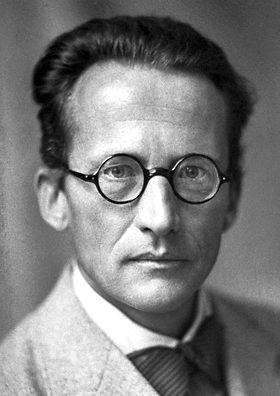
\includegraphics[width=\linewidth]{images/book3/schrodinger.jpg}
\end{minipage}\hfill
\begin{minipage}[t]{0.69\linewidth}\vspace{0pt}
{\small 薛定谔于 1926 年提出波动方程，该方程对氢原子的解即本章所述的轨道，
并由其重新得到玻尔所假设的能级。
他于 1933 年与他人共享诺贝尔物理学奖。
（照片：诺贝尔基金会，公有领域，
维基共享资源。）}
\end{minipage}
\end{omfigure}

\section{径向部分}

电子位于半径分别为 $r$ 与 $r +
dr$ 的两球面之间的概率，等于 $|\psi|^2$ 在体积为 $4\pi r^2\,dr$ 的球壳上的积分；对任一轨道，
在角度积分之后，其为 $r^2R^2\,dr$。

\begin{definition}[径向分布]\label{def:b2:atomic-orbitals:radial-distribution}
轨道的\emph{径向分布函数}\index{径向分布函数}
为 $P(r) = r^2R_{nl}(r)^2$：$P(r)\,dr$ 为电子位于
距原子核 $r$ 与 $r + dr$ 之间的概率。\emph{最概然
半径}\index{最概然半径}是其最大峰处的 $r$ 值。
\end{definition}

\begin{proposition}[1s 的归一化]\label{prop:b2:atomic-orbitals:normalised}
$\int_0^\infty P_{1s}(r)\,dr = 1$.
\end{proposition}

\begin{proof}
取 $Z = 1$，$r$ 以 $a_0$ 为单位，则 $P_{1s} = 4r^2\mathrm e^{-2r}$。两次分部积分，
$\int_0^\infty r^2\mathrm e^{-2r}\,dr = \frac22\int_0^\infty r\,\mathrm e^{-2r}\,dr =
\frac12\int_0^\infty\mathrm e^{-2r}\,dr = \frac14$，且 $4 \times \frac14 = 1$。
\end{proof}

\begin{proposition}[最概然半径]\label{prop:b2:atomic-orbitals:most-probable}
对于 1s 轨道，最概然半径为 $a_0/Z$。对于 $l =
n - 1$ 的轨道（1s、2p、3d、\dots），其为 $n^2a_0/Z$。
\end{proposition}

\begin{proof}
对于 $l = n - 1$，径向部分无节点：$R \propto \rho^{n-1}\mathrm e^{-\rho/n}$，
故 $P \propto \rho^{2n}\mathrm e^{-2\rho/n}$，$d\ln P/d\rho = 2n/\rho - 2/n$，并在
$\rho = n^2$ 处为零，即 $r = n^2a_0/Z$。当 $n = 1$ 时，$r = a_0/Z$。
\end{proof}

\begin{proposition}[1s 电子的平均半径]\label{prop:b2:atomic-orbitals:mean-radius}
1s 电子到原子核的平均距离为 $\langle r\rangle = 3a_0/(2Z)$，
大于其最概然半径。
\end{proposition}

\begin{proof}
取 $Z = 1$，则 $\langle r\rangle = \int_0^\infty r\,P(r)\,dr = 4\int_0^\infty r^3\mathrm e^{-2r}
\,dr = 4 \times 3!/2^4 = 3/2$。分布在 $r$ 很大时有一条长尾，
这使平均值超过极大值所在的位置。
\end{proof}

\begin{definition}[节点]\label{def:b2:atomic-orbitals:node}
原子轨道的\emph{节面}\index{节面}是这样一个曲面，
其上波函数为零且改变符号。它是\emph{径向节点}\index{径向节点}
（球面），当径向部分为零时；一个\emph{角向
节面}\index{角向节面}（过原子核的平面或锥面）
在角向部分为零时出现。
\end{definition}

\begin{proposition}[节点计数]\label{prop:b2:atomic-orbitals:nodes}
轨道 $(n, l)$ 有 $n - l - 1$ 个径向节点和 $l$ 个角向节面，总计
$n - 1$ 个。
\end{proposition}

\begin{proof}
对\cref{thm:b2:atomic-orbitals:hydrogen}中的函数：$R_{2s}$ 在
$\rho = 2$ 处为零，$R_{3s}$ 在 $2\rho^2 - 18\rho + 27$ 的两根（$\rho = 1.90$ 与 $7.10$）处为零，
$R_{3p}$ 在 $\rho = 6$ 处为零；$R_{1s}$、$R_{2p}$、$R_{3d}$ 均不为零。角向部分
对 p 轨道在一个平面上为零（即 $z = 0$，对应 $p_z$），对 d 轨道则在两个
平面上为零，或对 $d_{z^2}$ 在一个锥面上为零。一般情形在本阶段不加证明地承认。
\end{proof}

\begin{omfigure}
\begin{tikzpicture}
\begin{axis}[width=0.55\linewidth, height=6cm, xmin=0, xmax=24, ymin=0, ymax=0.58,
  axis x line=bottom, axis y line=left, xlabel={$r/a_0$}, ylabel={$P(r)$},
  tick label style={font=\small}, label style={font=\small}, title={\small 径向分布，$Z = 1$}]
\addplot[omThm, thick] table[x=r, y=s1] {figdata/out/bachelor-2-atomic-orbitals-a.dat};
\addplot[omDef, thick] table[x=r, y=s2] {figdata/out/bachelor-2-atomic-orbitals-a.dat};
\addplot[omDef, thick, dashed] table[x=r, y=p2] {figdata/out/bachelor-2-atomic-orbitals-a.dat};
\addplot[omProp, thick] table[x=r, y=s3] {figdata/out/bachelor-2-atomic-orbitals-a.dat};
\addplot[omProp, thick, dashed] table[x=r, y=p3] {figdata/out/bachelor-2-atomic-orbitals-a.dat};
\addplot[omProp, thick, dotted] table[x=r, y=d3] {figdata/out/bachelor-2-atomic-orbitals-a.dat};
\node[font=\scriptsize, omThm, anchor=west] at (axis cs:1.4,0.53) {1s};
\node[font=\scriptsize, omDef, anchor=south] at (axis cs:4.0,0.215) {2p};
\node[font=\scriptsize, omDef, anchor=south west] at (axis cs:6.4,0.17) {2s};
\node[font=\scriptsize, omProp, anchor=south] at (axis cs:10.5,0.12) {3d};
\node[font=\scriptsize, omProp, anchor=west] at (axis cs:17,0.085) {3s, 3p};
\end{axis}
\end{tikzpicture}\hfill
\begin{tikzpicture}
\begin{axis}[width=0.42\linewidth, height=6cm, xmin=0, xmax=20, ymin=-0.12, ymax=0.75,
  axis x line=middle, axis y line=left, xlabel={$r/a_0$}, ylabel={$R$},
  tick label style={font=\small}, label style={font=\small}, title={\small 径向部分}]
\addplot[omDef, thick] table[x=r, y=R2s] {figdata/out/bachelor-2-atomic-orbitals-b.dat};
\addplot[omProp, thick] table[x=r, y=R3s] {figdata/out/bachelor-2-atomic-orbitals-b.dat};
\node[font=\scriptsize, omDef, anchor=west] at (axis cs:0.4,0.62) {$R_{2s}$};
\node[font=\scriptsize, omProp, anchor=west] at (axis cs:0.6,0.30) {$R_{3s}$};
\node[font=\scriptsize, anchor=south west] at (axis cs:3,0.15) {节点};
\draw[thin, ->] (axis cs:3,0.15) -- (axis cs:2.05,0.01);
\end{axis}
\end{tikzpicture}

{\small 左：氢原子各轨道的径向分布 $P(r) = r^2R^2$，
直至 $n = 3$；$n$ 越大，电子离核越远，s 轨道
有较小的内侧极大值（穿透效应）。右：$R_{2s}$ 与 $R_{3s}$ 在其
径向节点处变号（$r = 2a_0$；$1.90a_0$ 与 $7.10a_0$）。}
\end{omfigure}

\begin{omfigure}
\begin{tikzpicture}
\begin{axis}[scale only axis, width=0.32\linewidth, height=0.32\linewidth,
  xmin=-6, xmax=6, ymin=-6, ymax=6, axis lines=none, title={\small 1s}]
\addplot[only marks, mark=*, mark size=0.25pt, omDef] table[x=x, y=y] {figdata/out/bachelor-2-atomic-orbitals-c-1s.dat};
\end{axis}
\end{tikzpicture}\hspace{0.12\linewidth}%
\begin{tikzpicture}
\begin{axis}[scale only axis, width=0.32\linewidth, height=0.32\linewidth,
  xmin=-14, xmax=14, ymin=-14, ymax=14, axis lines=none, title={\small 2s}]
\addplot[only marks, mark=*, mark size=0.25pt, omDef] table[x=x, y=y] {figdata/out/bachelor-2-atomic-orbitals-c-2s.dat};
\draw[densely dashed, omThm] (axis cs:0,0) circle[radius=2];
\end{axis}
\end{tikzpicture}

{\small 氢原子 1s 与 2s 轨道在过原子核的一个平面内的点密度图：
点的密度遵循 $|\psi|^2$（确定性
抽样）。2s 电子云中有一个空环，即位于 $2a_0$ 处的径向节点（虚线）；
图框宽度分别为 12 与 28 $a_0$。}
\end{omfigure}

\section{角向部分}

角向部分决定形状。s 轨道呈球形；p 轨道沿其轴有两个
符号相反的瓣，由一个节面隔开；d 轨道有
四个符号交替的瓣（对于 $d_{z^2}$，为两个瓣和一个环）。瓣的
符号本身没有物理意义——$\psi$ 与 $-\psi$ 描述同一
状态——但两个轨道的相对符号，在下一章中
决定它们能否成键。

\begin{omfigure}
\begin{tikzpicture}[font=\small]
  \pic at (0,0) {oms={1}};
  \node[below] at (0,-0.75) {s};
  \pic at (2.0,0) {omp={1}{0}};
  \draw[->, black!55, thin] (1.0,0) -- (3.0,0) node[right, font=\tiny] {$x$};
  \node[below] at (2.0,-0.75) {$\mathrm p_x$};
  \pic at (4.2,0) {omp={1}{90}};
  \draw[->, black!55, thin] (4.2,-0.95) -- (4.2,0.95) node[above, font=\tiny] {$z$};
  \node[below] at (4.75,-0.75) {$\mathrm p_z$};
  \pic at (6.6,0) {omdxy}; \node[below] at (6.6,-1.0) {$\mathrm d_{xy}$};
  \pic at (9.0,0) {omdx2y2}; \node[below] at (9.0,-1.0) {$\mathrm d_{x^2-y^2}$};
  \pic at (11.4,0) {omdz2}; \node[below] at (11.4,-1.0) {$\mathrm d_{z^2}$};
\end{tikzpicture}

{\small 真实原子轨道示意图：瓣表示 $|\psi|$
较大的区域，颜色由 $\psi$ 的符号决定（蓝色为正，橙色为负）。
$\mathrm d_{xz}$ 和 $\mathrm d_{yz}$ 轨道的形状与 $\mathrm d_{xy}$ 相同，位于
其名称所指的平面内。}
\end{omfigure}

\begin{method}[由量子数画原子轨道示意图]\label{met:b2:atomic-orbitals:draw-orbital}
\begin{enumerate}
  \item 由 $l$ 定形状：s 为球形，p 为两瓣，d 为四瓣（
        对 $d_{z^2}$ 为两瓣加一圆环）；由下标定取向。
  \item 数出 $l$ 个角向节面（过原子核的平面），
        并使相邻的瓣符号相反。
  \item 数出 $n - l - 1$ 个径向节点：主瓣内侧
        符号相反的内层（画示意图时通常省略）。
  \item 按 $n^2a_0/Z$ 确定大小：$n$ 越大，轨道越大；$Z$ 越大，轨道越小。
\end{enumerate}
\end{method}

\section{多电子原子}

在含有多个电子的原子中，每个电子感受到的原子核电荷都会
被其他电子屏蔽。原子轨道保持氢原子轨道的形状，
只是用有效核电荷 $Z^*$ 代替 $Z$，亚层能量现在取决于 $l$，
也取决于 $n$：s 电子的径向分布在靠近原子核处有内侧极大值，
因而所受屏蔽比同一电子层的 p 电子小，p 电子又比
d 电子小。

\begin{definition}[斯莱特规则]\label{def:b2:atomic-orbitals:slater}
\emph{斯莱特规则}\index{斯莱特规则}估算电子所感受的有效核电荷
$Z^* = Z - \sigma$。电子分组如下：
（1s）（2s、2p）（3s、3p）（3d）（4s、4p）（4d）（4f）（5s、5p）\dots；
某电子的屏蔽常数 $\sigma$ 为其他各电子贡献之和：
与其同组的每个其他电子贡献 0.35（1s 中为 0.30）；
对 s 或 p 电子，电子层 $n - 1$ 中每个电子贡献 0.85，
更低电子层中每个电子贡献 1.00；对 d 或 f 电子，其下方各组中
每个电子贡献 1.00。位于上方的各组不贡献。
\end{definition}

\begin{omfigure}
\small
\renewcommand{\arraystretch}{1.2}
\begin{tabular}{l|ccccc}
被研究电子 & 同组 & 电子层 $n - 1$ & 更低电子层 & 上方各组 \\ \hline
1s & 0.30 & --- & --- & 0 \\
$n$s, $n$p & 0.35 & 0.85 & 1.00 & 0 \\
$n$d, $n$f & 0.35 & 1.00 & 1.00 & 0 \\
\end{tabular}

\smallskip
{\small 斯莱特屏蔽常数，按每个屏蔽电子计。有效
主量子数依次为 $n^* = 1, 2, 3, 3.7, 4.0, 4.2$，对应 $n = 1$ 至 6。}
\end{omfigure}

\begin{method}[计算有效核电荷]\label{met:b2:atomic-orbitals:slater}
\begin{enumerate}
  \item 按 $n$ 的顺序把电子排布写成斯莱特分组：
        s 与 p 同组，d 与 f 分开。
  \item 选定电子，同组中每个其他电子加 0.35。
  \item 对紧邻其下的电子层中每个电子，s 或 p 电子加 0.85（d 或 f 电子加 1.00），
        更深层中每个电子加 1.00。
  \item $Z^* = Z - \sigma$.
\end{enumerate}
\end{method}

\begin{definition}[轨道能量与半径]\label{def:b2:atomic-orbitals:orbital-energy}
在斯莱特模型中，电子的\emph{轨道能量}\index{轨道能量}
由其有效核电荷 $Z^*$ 与有效主量子数 $n^*$ 决定，
为 $\varepsilon = -E_RZ^{*2}/n^{*2}$；其\emph{轨道半径}\index{轨道半径}
为 $n^{*2}a_0/Z^*$，即电荷为
$Z^*$ 的类氢轨道的最概然半径。
\end{definition}

\begin{proposition}[斯莱特能量]\label{prop:b2:atomic-orbitals:slater-energy}
由 $k$ 个有效核电荷为 $Z^*$ 的电子组成的一组，其能量近似为
$k\varepsilon = -kE_RZ^{*2}/n^{*2}$，原子的总电子能量
等于其各组能量之和。
\end{proposition}

\admitted

\begin{example}[铁：先填 4s 还是 3d？]\label{ex:b2:atomic-orbitals:iron}
铁为 $[\ce{Ar}]\,3\mathrm d^6\,4\mathrm s^2$。对一个 4s 电子：$\sigma = 0.35 + 14
\times 0.85 + 10 \times 1.00 = 22.25$, $Z^* = 3.75$, $\varepsilon = -13.6 \times
3.75^2/3.7^2 = \qty{-14.0}{eV}$。对一个 3d 电子：$\sigma = 5 \times 0.35 + 18 \times 1.00 =
19.75$，$Z^* = 6.25$，$\varepsilon = -13.6 \times 6.25^2/9 = \qty{-59}{eV}$。
3d 电子束缚得紧得多：虽然在构造顺序中 4s 先被填充，
但铁电离时失去的是一个 4s 电子，因此
亚铁离子的电子排布为 $[\ce{Ar}]\,3\mathrm d^6$。
\end{example}

\section{轨道能量与大小的应用}

\begin{proposition}[由斯莱特能量求电离能]\label{prop:b2:atomic-orbitals:ionisation}
在斯莱特模型中，原子的第一电离能为
离子与原子总能量之差，按组计算，
各组使用其自身的有效核电荷。
\end{proposition}

\begin{proof}
电离能为 $E(\text{离子}) - E(\text{原子})$；由
\cref{prop:b2:atomic-orbitals:slater-energy}，二者均为各组能量之和，且
只有失去电子的那一组发生改变（内层各组
不受外层电子屏蔽）。
\end{proof}

\begin{example}[碳]\label{ex:b2:atomic-orbitals:carbon}
碳，（2s、2p）$^4$：$Z^* = 6 - 2 \times 0.85 - 3 \times 0.35 = 3.25$；该组能量为
$4 \times (-13.6 \times 3.25^2/4) = \qty{-143.6}{eV}$。离子 \ce{C+}，（2s、2p）$^3$：$Z^* =
3.60$，$3 \times (-13.6 \times 3.60^2/4) = \qty{-132.2}{eV}$。电离能为
\qty{11.5}{eV}，实测值为 \qty{11.26}{eV}。
% ledger: ie:C, const:RyhcEV
\end{example}

\begin{omfigure}
\begin{tikzpicture}
\begin{axis}[width=0.47\linewidth, height=5.4cm, xmin=0.5, xmax=8.5, ymin=0, ymax=6.5,
  axis x line=bottom, axis y line=left, xtick={1,2,3,4,5,6,7,8},
  xticklabels={Li,Be,B,C,N,O,F,Ne}, tick label style={font=\small},
  label style={font=\small}, title={\small 第二周期}]
\addplot[omThm, thick, mark=*, mark size=1.3pt] table[x=k, y=zs] {figdata/out/bachelor-2-atomic-orbitals-d-period.dat};
\addplot[omDef, thick, mark=square*, mark size=1.3pt] table[x=k, y=r] {figdata/out/bachelor-2-atomic-orbitals-d-period.dat};
\node[font=\scriptsize, omThm, anchor=south east] at (axis cs:7.8,5.3) {$Z^*$};
\node[font=\scriptsize, omDef, anchor=south west] at (axis cs:1.2,3.1) {半径（$a_0$）};
\end{axis}
\end{tikzpicture}\hfill
\begin{tikzpicture}
\begin{axis}[width=0.47\linewidth, height=5.4cm, xmin=1.5, xmax=6.5, ymin=0, ymax=9,
  axis x line=bottom, axis y line=left, xtick={2,3,4,5,6},
  xticklabels={Li,Na,K,Rb,Cs}, tick label style={font=\small},
  label style={font=\small}, title={\small 第 1 族}]
\addplot[omThm, thick, mark=*, mark size=1.3pt] table[x=n, y=zs] {figdata/out/bachelor-2-atomic-orbitals-d-group.dat};
\addplot[omDef, thick, mark=square*, mark size=1.3pt] table[x=n, y=r] {figdata/out/bachelor-2-atomic-orbitals-d-group.dat};
\node[font=\scriptsize, omThm, anchor=north] at (axis cs:4,2.0) {$Z^*$};
\node[font=\scriptsize, omDef, anchor=west] at (axis cs:2.1,5.4) {半径（$a_0$）};
\end{axis}
\end{tikzpicture}

{\small 价电子的斯莱特有效核电荷与轨道半径
$n^{*2}a_0/Z^*$。沿第二周期，$Z^*$ 每增加一个元素增大 0.65，原子
随之收缩；沿第 1 族向下，$Z^*$ 维持在 1.30 继而 2.20，而 $n^*$ 增大，原子
随之膨胀。}
\end{omfigure}

该模型重现了本科一年级分册中的周期性规律。沿周期方向，每
增加一个质子，与之同时增加的电子只屏蔽其 0.35：$Z^*$ 增大，
外层轨道收缩，结合也更牢固。沿族向下，$Z^*$ 几乎
不变，而外层电子层向外移：原子变大，电离能
降低。钠的 3s 电子 $Z^* = 2.20$，其轨道半径为
$9/2.2 = 4.1a_0$；氯的 3p 电子 $Z^* = 6.10$，半径为 $9/6.1 = 1.5a_0$。

\section{练习}

\begin{exercise}[$\star$]\label{exo:b2:atomic-orbitals:1}
给出 3p 轨道和 4d 轨道的量子数 $n$ 与 $l$，以及径向节点数和角向
节点数。
\end{exercise}

\begin{exercise}[$\star$]\label{exo:b2:atomic-orbitals:2}
由 $R_{2p}$ 证明：氢原子 2p 电子的最概然半径为
$4a_0$，并以皮米表示。
\end{exercise}

\begin{exercise}[$\star$]\label{exo:b2:atomic-orbitals:3}
计算氢原子 1s 电子出现在距原子核
小于 $a_0$ 处的概率。
\end{exercise}

\begin{exercise}[$\star$]\label{exo:b2:atomic-orbitals:4}
画出 $3\mathrm d_{xy}$ 轨道的示意图：瓣、符号、节面。它有多少个径向
节点？
\end{exercise}

\begin{exercise}[$\star\star$]\label{exo:b2:atomic-orbitals:5}
计算氧原子 2p 电子的斯莱特有效核电荷，以及由此得到的轨道
半径。
\end{exercise}

\begin{exercise}[$\star\star$]\label{exo:b2:atomic-orbitals:6}
以铁为例，说明为什么 \ce{Fe^3+} 的电子排布是
$[\ce{Ar}]\,3\mathrm d^5$，而不是 $[\ce{Ar}]\,3\mathrm d^3 4\mathrm s^2$。
\end{exercise}

\begin{exercise}[$\star\star$]\label{exo:b2:atomic-orbitals:7}
用斯莱特规则估算锂和钠的第一电离能，
并与实测值 5.39 和 \qty{5.14}{eV} 比较。加以评论。
\end{exercise}

\begin{exercise}[$\star\star$]\label{exo:b2:atomic-orbitals:8}
计算钠和氯最外层电子的 $Z^*$ 与轨道半径，
并说明钠原子为何更大。
\end{exercise}

\begin{exercise}[$\star\star$]\label{exo:b2:atomic-orbitals:9}
证明氢原子的 1s 轨道与 2s 轨道正交，即
$\int\psi_{1s}\psi_{2s}\,dV = 0$。
\end{exercise}

\begin{exercise}[$\star\star\star$]\label{exo:b2:atomic-orbitals:10}
写出 $R_{2p} = N\rho\,\mathrm e^{-\rho/2}$，并求使其归一化的常数 $N$
（$Z = 1$，$r$ 以 $a_0$ 为单位）。
\end{exercise}

\begin{exercise}[$\star\star\star$]\label{exo:b2:atomic-orbitals:11}
比较 1s 电子的平均半径与最概然半径，并
根据 $P(r)$ 的形状说明二者为何不同。
\end{exercise}

\begin{exercise}[$\star\star\star$]\label{exo:b2:atomic-orbitals:12}
求 $\mathrm p_z$ 轨道的节面，并证明 $\psi_{2p_z}$
在越过节面时变号。该节面上的概率密度是多少？
\end{exercise}

\section{问题：电子在哪里？}

\begin{problem}[{周末问题——氢原子的 1s 轨道及其半径，
在给定距离之外找到电子的概率，2s 与 2p 的节点和
极大值，以及用斯莱特规则估算碳、
氮、氧的电离能}]
\label{pb:b2:atomic-orbitals:1}
数据：$a_0 = \qty{52.9}{pm}$；$E_R = \qty{13.6}{eV}$；实测第一电离
能（\unit{eV}）：C 11.26，N 14.53，O 13.62。$\psi_{1s} = \pi^{-1/2}a_0^{-3/2}\,
\mathrm e^{-r/a_0}$。
% ledger: const:a0, const:RyhcEV, ie:C, ie:N, ie:O

\medskip
\noindent\textbf{第一部分——1s 轨道。}
\begin{enumerate}
  \item 验证 $\psi_{1s}$ 已归一化（取 $dV = 4\pi r^2\,dr$）。
  \item 写出径向分布函数 $P(r)$。
  \item 求最概然半径。
  \item 计算平均半径。
  \item 为什么平均半径大于最概然半径？
  \item 概率密度在原子核处最大，而 $P(0) = 0$。
        请解释。
  \item 以皮米为单位，给出最概然半径。
\end{enumerate}

\medskip
\noindent\textbf{第二部分——超出某一半径。}
\begin{enumerate}[resume]
  \item 证明：电子位于距离大于 $r_0 =
        xa_0$ 处的概率为 $\mathrm e^{-2x}(1 + 2x + 2x^2)$。
  \item 计算 $r_0 = a_0$ 时的概率。
  \item 计算 $r_0 = 2a_0$ 时的概率。
  \item 用试算法求出球的半径，使电子处于该球内的
        概率为 0.90。
  \item 原子在何种意义上没有边界，又在何种意义上具有大小？
\end{enumerate}

\medskip
\noindent\textbf{第三部分——2s 与 2p。}
\begin{enumerate}[resume]
  \item 给出 2s 与 2p 的节点（写出数目、类型与位置）。
  \item $R_{2s}$ 在何处改变符号？
  \item 求 2p 的最概然半径。
  \item 求 $P_{2s} \propto r^2(2 - r)^2\mathrm e^{-r}$ 的两个极大值（$r$ 以
        $a_0$ 为单位）。
  \item 2s 与 2p 中，哪一个的电子密度更靠近原子核？这对多电子原子
        意味着什么？
  \item 对类氢离子 \ce{C^5+}，这些半径如何变化？
\end{enumerate}

\medskip
\noindent\textbf{第四部分——碳、氮、氧。}
\begin{enumerate}[resume]
  \item 计算 C、N、O 中 2p 电子的斯莱特 $Z^*$。
  \item 计算相应的轨道能量。
  \item 将碳的第一电离能估算为各组
        能量之差。
  \item 氮的情形相同。
  \item 氧的情形相同，并将三者与实测值比较。
  \item 模型遗漏了实测值的哪一特征？原因何在？
  \item 给出氢原子 1s 电子位于距离大于
        $2a_0$ 处的概率。
\end{enumerate}
\end{problem}
